\documentclass{beamer}
\usetheme{Madrid}
\usecolortheme{default}
\usepackage{tikz}
\usetikzlibrary{shapes}
\usepackage{amsmath}
\usepackage{booktabs}

% Title page information
\title{Causal Reasoning: Understanding Why Things Happen}
\subtitle{Introduction to Logic}
\author{Brendan Shea, PhD}
\date{}

\begin{document}
	
	% Title slide
	\frame{\titlepage}
	
	% Slide 1: Causal Reasoning: Understanding Why Things Happen
	\begin{frame}{Causal Reasoning: Understanding Why Things Happen}
		\begin{itemize}
			\item \textbf{Causal reasoning} is the process of identifying relationships where one event or condition brings about another.
			\item We use causal thinking every day when we ask "why" questions: Why did my car break down? Why did I get sick?
			\item Understanding causation helps us predict future events and make better decisions in our personal and professional lives.
			\item Today we'll learn systematic methods to distinguish genuine causes from mere coincidences.
		\end{itemize}
		
		\begin{block}{Key Question}
			How can we reliably determine what causes what in a complex world?
		\end{block}
	\end{frame}
	
	% Slide 2: From Correlation to Causation: Today's Journey
	\begin{frame}{From Correlation to Causation: Today's Journey}
		\begin{itemize}
			\item \textbf{Correlation} means two things tend to occur together, but this doesn't necessarily mean one causes the other.
			\item The famous phrase "correlation does not imply causation" warns us against jumping to conclusions about cause and effect.
			\item We'll explore scientific methods that help us move beyond correlation to establish genuine causal relationships.
			\item By the end of this lecture, you'll have tools to critically evaluate causal claims in media, research, and everyday life.
		\end{itemize}
		
		\begin{alertblock}{Warning}
			Many false beliefs arise from mistaking correlation for causation!
		\end{alertblock}
	\end{frame}
	
	% Slide 3: Why Causal Thinking Matters in Logic and Life
	\begin{frame}{Why Causal Thinking Matters in Logic and Life}
		\begin{itemize}
			\item Causal reasoning connects to our previous studies of deductive, inductive, and abductive reasoning.
			\item In science, establishing causation is essential for developing effective treatments, policies, and technologies.
			\item Understanding causation helps us avoid superstitious thinking and make rational decisions based on evidence.
			\item Causal literacy is crucial for being an informed citizen who can evaluate claims about health, economics, and social issues.
		\end{itemize}
		
		\begin{example}[Real-World Applications]
			\begin{itemize}
				\item Does this medication actually cure the disease?
				\item Will this economic policy reduce unemployment?
				\item Does violent media cause aggressive behavior?
			\end{itemize}
		\end{example}
	\end{frame}
	
	% Slide 4: Defining Causation: The Interventionist Approach
	\begin{frame}{Defining Causation: The Interventionist Approach}
		\begin{itemize}
			\item The \textbf{interventionist approach} defines causation in terms of what would happen if we actively changed something.
			\item X causes Y if intervening to change X would lead to a change in Y, all else being equal.
			\item This approach emphasizes that causes are things we can manipulate or that could be manipulated in principle.
			\item The key insight is that causation is about what happens when we "wiggle" one variable and observe effects on another.
		\end{itemize}
		
		\begin{block}{Formal Definition}
			X causes Y if and only if there exists an intervention on X that would change Y (holding all else constant).
		\end{block}
	\end{frame}
	
	% Slide 5: "If I Do X, Then Y Happens": Intervention in Action
	\begin{frame}{"If I Do X, Then Y Happens": Intervention in Action}
		\begin{itemize}
			\item \textbf{Intervention} means actively changing a variable rather than just observing it naturally occur.
			\item When we flip a light switch (intervention on X), the light turns on (change in Y) - this suggests a causal relationship.
			\item The intervention must be "surgical" - it changes only the target variable without affecting other factors directly.
			\item This approach helps us distinguish causation from mere association or correlation in data.
		\end{itemize}
		
		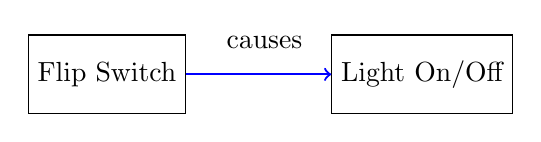
\begin{tikzpicture}[scale=0.8]
			% Draw boxes
			\node[draw, rectangle, minimum width=2cm, minimum height=1cm] (X) at (0,0) {Flip Switch};
			\node[draw, rectangle, minimum width=2cm, minimum height=1cm] (Y) at (5,0) {Light On/Off};
			
			% Draw arrow
			\draw[->, thick, blue] (X) -- (Y);
			
			% Label
			\node at (2.5, 0.5) {causes};
		\end{tikzpicture}
	\end{frame}
	
	% Slide 6: Counterfactual Thinking: "What If Things Were Different?"
	\begin{frame}{Counterfactual Thinking: "What If Things Were Different?"}
		\begin{itemize}
			\item \textbf{Counterfactual reasoning} asks what would have happened if circumstances had been different.
			\item "The rock caused the window to break" means: if the rock hadn't been thrown, the window wouldn't have broken.
			\item This approach defines causation by comparing the actual world with hypothetical alternative worlds.
			\item Counterfactuals help us think about causation even when we can't perform real interventions.
		\end{itemize}
		
		\begin{example}[Counterfactual Analysis]
			\begin{itemize}
				\item Actual world: I studied hard and passed the exam
				\item Counterfactual world: If I hadn't studied hard, I would have failed
				\item Conclusion: Studying hard caused me to pass
			\end{itemize}
		\end{example}
	\end{frame}
	
	% Slide 7: Example: Why Did Wile E. Coyote Fall? (Interventionist View)
	\begin{frame}{Example: Why Did Wile E. Coyote Fall? (Interventionist View)}
		\begin{itemize}
			\item In the cartoon, Wile E. Coyote runs off a cliff but doesn't fall until he looks down and realizes there's no ground.
			\item \textbf{Interventionist analysis}: If we intervened to prevent him from looking down, would he still fall?
			\item In reality, gravity causes the fall regardless of awareness - looking down is not the true cause.
			\item This example illustrates how the interventionist approach helps us identify genuine causes versus coincidental timing.
		\end{itemize}
		
		\begin{alertblock}{Cartoon vs. Reality}
			In cartoons: Looking down → Falling (not real causation!)\\
			In reality: Running off cliff → Falling (true causation)
		\end{alertblock}
	\end{frame}
	
	% Slide 8: Example: Would Batman Still Fight Crime Without His Parents' Death? (Counterfactual)
	\begin{frame}{Example: Would Batman Still Fight Crime Without His Parents' Death? (Counterfactual)}
		\begin{itemize}
			\item Batman's origin story claims his parents' murder caused him to become a crime fighter.
			\item \textbf{Counterfactual analysis}: In a world where his parents lived, would Bruce Wayne still become Batman?
			\item Most interpretations suggest no - he would likely have become a philanthropist or businessman instead.
			\item This example shows how counterfactuals help us evaluate causal claims in complex narratives where we can't intervene.
		\end{itemize}
		
		\begin{block}{Counterfactual Worlds}
			\begin{tabular}{l|l}
				\textbf{Actual World} & \textbf{Counterfactual World} \\
				\hline
				Parents murdered & Parents survive \\
				Becomes Batman & Remains civilian \\
				Fights crime & Runs Wayne Enterprises \\
			\end{tabular}
		\end{block}
	\end{frame}
	
	% Slide 9: Everyday Causation: Coffee and Alertness
	\begin{frame}{Everyday Causation: Coffee and Alertness}
		\begin{itemize}
			\item We often claim "coffee makes me alert," but how can we verify this causal relationship?
			\item \textbf{Intervention test}: When I drink coffee (intervention), I become more alert within 20-30 minutes.
			\item \textbf{Counterfactual test}: On days I skip coffee, I remain drowsy longer than on days I drink it.
			\item However, other factors like placebo effects, sleep quality, and time of day might also influence alertness.
		\end{itemize}
		
		\begin{example}[Personal Experiment]
			Try alternating coffee and decaf for a week while tracking alertness levels - this creates your own mini-intervention study!
		\end{example}
	\end{frame}
	
	% Slide 10: Multiple Causes: Why Your Phone Battery Dies
	\begin{frame}{Multiple Causes: Why Your Phone Battery Dies}
		\begin{itemize}
			\item Real-world events often have \textbf{multiple causes} working together rather than a single cause.
			\item Your phone battery dies because of: screen brightness, running apps, cellular signal strength, and battery age.
			\item Each factor contributes causally - intervening on any one of them would affect battery life.
			\item Understanding multiple causation helps us see why simple "X causes Y" statements often oversimplify reality.
		\end{itemize}
		
		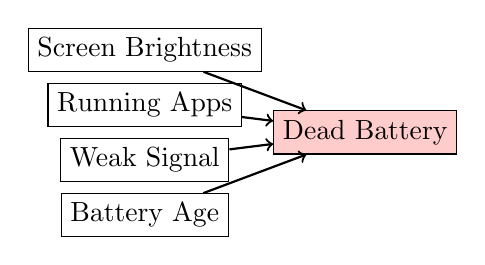
\begin{tikzpicture}[scale=0.7]
			% Multiple causes pointing to one effect
			\node[draw, rectangle] (brightness) at (-2, 1.5) {Screen Brightness};
			\node[draw, rectangle] (apps) at (-2, 0.5) {Running Apps};
			\node[draw, rectangle] (signal) at (-2, -0.5) {Weak Signal};
			\node[draw, rectangle] (age) at (-2, -1.5) {Battery Age};
			\node[draw, rectangle, fill=red!20] (dead) at (2, 0) {Dead Battery};
			
			% Arrows
			\draw[->, thick] (brightness) -- (dead);
			\draw[->, thick] (apps) -- (dead);
			\draw[->, thick] (signal) -- (dead);
			\draw[->, thick] (age) -- (dead);
		\end{tikzpicture}
	\end{frame}
	
	% Slide 11: The Correlation Trap: When Association Isn't Causation
	\begin{frame}{The Correlation Trap: When Association Isn't Causation}
		\begin{itemize}
			\item \textbf{The correlation trap} occurs when we mistake statistical association for causal relationship.
			\item Just because two things occur together frequently doesn't mean one causes the other.
			\item Classic example: Ice cream sales and drowning deaths both increase in summer, but ice cream doesn't cause drowning!
			\item The trap is especially dangerous when correlation confirms our existing beliefs or desires.
		\end{itemize}
		
		\begin{alertblock}{Remember}
			Correlation is evidence that might suggest causation, but it's not proof! Always look for alternative explanations.
		\end{alertblock}
	\end{frame}
	
	% Slide 12: Confounding Variables: Hidden Factors at Play
	\begin{frame}{Confounding Variables: Hidden Factors at Play}
		\begin{itemize}
			\item A \textbf{confounding variable} is a hidden factor that influences both the supposed cause and effect.
			\item Confounders create the illusion of causation where none exists by making two things appear related.
			\item Example: Cities with more firefighters have more fires, but firefighters don't cause fires - large city size causes both!
			\item Identifying and controlling for confounders is crucial for accurate causal inference.
		\end{itemize}
		
		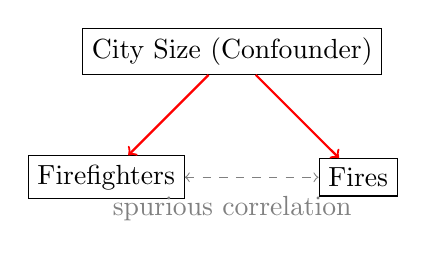
\begin{tikzpicture}[scale=0.8]
			% Nodes
			\node[draw, rectangle] (conf) at (2, 2) {City Size (Confounder)};
			\node[draw, rectangle] (x) at (0, 0) {Firefighters};
			\node[draw, rectangle] (y) at (4, 0) {Fires};
			
			% Arrows from confounder
			\draw[->, thick, red] (conf) -- (x);
			\draw[->, thick, red] (conf) -- (y);
			
			% Dotted line showing spurious correlation
			\draw[<->, dashed, gray] (x) -- (y);
			\node[gray] at (2, -0.5) {spurious correlation};
		\end{tikzpicture}
	\end{frame}
	
	% Slide 13: Example: Ice Cream Sales and Drowning Deaths
	\begin{frame}{Example: Ice Cream Sales and Drowning Deaths}
		\begin{itemize}
			\item Data shows that when ice cream sales increase, drowning deaths also increase - but ice cream doesn't cause drowning!
			\item The hidden \textbf{confounding variable} is temperature/season: hot weather causes both more ice cream consumption and more swimming.
			\item This example perfectly illustrates why "correlation does not imply causation" is such an important principle.
			\item Without considering confounders like weather, we might implement useless policies like banning ice cream to prevent drowning.
		\end{itemize}
		
		\begin{block}{The Real Causal Structure}
			\begin{center}
				Hot Weather → More Ice Cream Sales\\
				Hot Weather → More Swimming → More Drowning Risk\\
				(No direct causal link between ice cream and drowning!)
			\end{center}
		\end{block}
	\end{frame}
	
	% Slide 14: Simpson's Paradox: When Data Misleads
	\begin{frame}{Simpson's Paradox: When Data Misleads}
		\begin{itemize}
			\item \textbf{Simpson's Paradox} occurs when a trend appears in different groups of data but disappears or reverses when groups are combined.
			\item Example: A treatment might appear harmful overall but actually be beneficial within each patient subgroup.
			\item This paradox shows how aggregating data can hide true causal relationships and lead to wrong conclusions.
			\item The paradox typically arises when we ignore an important variable that affects both treatment assignment and outcomes.
		\end{itemize}
		
		\begin{example}[University Admissions]
			\small{Women have higher admission rates in each department but lower overall!}
			\\
			\begin{tabular}{l|c|c}
				Department & Male Admit Rate & Female Admit Rate \\
				\hline
				Engineering & 30\% & 35\% \\
				Liberal Arts & 60\% & 65\% \\
				\hline
				Overall & 45\% & 40\% \\
			\end{tabular}
			
		\end{example}
	\end{frame}
	
	% Slide 15: Fictional Example: Did Spider-Man's Powers Cause His Problems?
	\begin{frame}{Fictional Example: Did Spider-Man's Powers Cause His Problems?}
		\begin{itemize}
			\item Peter Parker gains powers and then experiences many personal tragedies - did the powers cause his problems?
			\item Alternative explanation: His decision to become a hero (not the powers themselves) puts him in dangerous situations.
			\item Another factor: "Parker Luck" suggests he was already prone to misfortune before gaining powers.
			\item This example shows how even in fiction, identifying true causes requires careful analysis of competing explanations.
		\end{itemize}
		
		\begin{alertblock}{Causal Analysis}
			Powers → Hero Choice → Dangerous Situations → Problems\\
			(The powers are only an indirect cause through Peter's choices!)
		\end{alertblock}
	\end{frame}
	
	% Slide 16: Selection Bias: Why Your Sample Matters
	\begin{frame}{Selection Bias: Why Your Sample Matters}
		\begin{itemize}
			\item \textbf{Selection bias} occurs when the sample we study isn't representative of the population we want to understand.
			\item Example: Studying only gym members to determine if exercise improves health ignores that healthier people might choose to join gyms.
			\item This bias can make us think we've found a causal relationship when we've actually just selected a special group.
			\item Selection bias is especially tricky because it can be invisible - we don't see the data we didn't collect.
		\end{itemize}
		
		\begin{example}[Survivor Bias in WWII]
			Engineers wanted to add armor where returning planes had bullet holes, but statistician Abraham Wald realized they should armor where the holes \textit{weren't} - those planes didn't return!
		\end{example}
	\end{frame}
	
	% Slide 17: The Gold Standard: Randomized Controlled Trials
	\begin{frame}{The Gold Standard: Randomized Controlled Trials}
		\begin{itemize}
			\item \textbf{Randomized Controlled Trials (RCTs)} are considered the gold standard for establishing causation.
			\item In an RCT, participants are randomly assigned to either receive a treatment or be in a control group.
			\item Random assignment ensures that confounding variables are distributed equally between groups on average.
			\item By comparing outcomes between treatment and control groups, we can isolate the causal effect of the treatment.
		\end{itemize}
		
		\begin{block}{Why RCTs Work}
			Randomization breaks the link between confounders and treatment assignment, allowing us to measure true causal effects.
		\end{block}
	\end{frame}
	
	% Slide 18: Key Components: Treatment, Control, and Randomization
	\begin{frame}{Key Components: Treatment, Control, and Randomization}
		\begin{itemize}
			\item \textbf{Treatment group} receives the intervention we're testing (new drug, teaching method, therapy, etc.).
			\item \textbf{Control group} receives either no treatment, a placebo, or the standard existing treatment.
			\item \textbf{Randomization} uses chance (like flipping a coin) to assign participants to groups, eliminating selection bias.
			\item These three components work together to create a fair comparison that reveals causal effects.
		\end{itemize}
		
		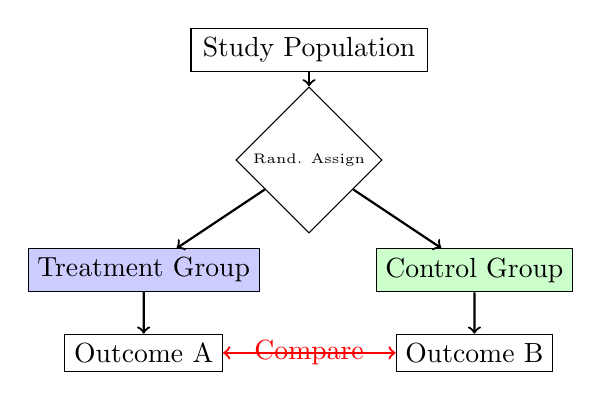
\begin{tikzpicture}[scale=0.7]
			% Population
			\node[draw, rectangle, minimum width=3cm] (pop) at (0, 2) {Study Population};
			
			% Randomization - SMALLER DIAMOND
			\node[draw, diamond, minimum size=1cm, inner sep=2pt] (rand) at (0, 0) {\tiny Rand. Assign};
			
			% Groups
			\node[draw, rectangle, fill=blue!20] (treat) at (-3, -2) {Treatment Group};
			\node[draw, rectangle, fill=green!20] (control) at (3, -2) {Control Group};
			
			% Outcomes
			\node[draw, rectangle] (out1) at (-3, -3.5) {Outcome A};
			\node[draw, rectangle] (out2) at (3, -3.5) {Outcome B};
			
			% Arrows
			\draw[->, thick] (pop) -- (rand);
			\draw[->, thick] (rand) -- (treat);
			\draw[->, thick] (rand) -- (control);
			\draw[->, thick] (treat) -- (out1);
			\draw[->, thick] (control) -- (out2);
			
			% Comparison
			\draw[<->, thick, red] (out1) -- (out2);
			\node[red] at (0, -3.5) {Compare};
		\end{tikzpicture}
		
		
	\end{frame}
	
	% Slide 19: Example: Testing Popeye's Spinach Hypothesis
	\begin{frame}{Example: Testing Popeye's Spinach Hypothesis}
		\begin{itemize}
			\item Popeye claims spinach causes super strength - how would we test this claim with an RCT?
			\item \textbf{Design}: Randomly assign 100 sailors to eat either spinach (treatment) or lettuce (control) daily for one month.
			\item \textbf{Measurement}: Test grip strength, lifting capacity, and endurance before and after the trial.
			\item \textbf{Result}: If the spinach group shows significantly greater strength gains, we have evidence for causation.
		\end{itemize}
		
		\begin{example}[RCT Design for Popeye]
			\small
			\begin{enumerate}
				\item Recruit 100 sailors of similar baseline strength
				\item Randomly assign: 50 to spinach, 50 to lettuce
				\item Both groups eat identical diets except for the vegetable
				\item Measure strength changes after 30 days
				\item Compare average improvements between groups
			\end{enumerate}
		\end{example}
	\end{frame}
	
	% Slide 20: The Placebo Effect: Mind Over Matter
	\begin{frame}{The Placebo Effect: Mind Over Matter}
		\begin{itemize}
			\item The \textbf{placebo effect} occurs when people improve simply because they believe they're receiving treatment.
			\item This psychological phenomenon can create false impressions of causation if not properly controlled.
			\item That's why control groups often receive a placebo (fake treatment) that looks identical to the real treatment.
			\item By comparing real treatment to placebo, we can separate the actual causal effect from psychological expectations.
		\end{itemize}
		
		\begin{block}{Example: Sugar Pills}
			In drug trials, the control group receives sugar pills that look identical to the real medication. Any improvement in the control group is due to placebo effect, not the drug's chemistry.
		\end{block}
	\end{frame}
	
	% Slide 21: Real Example: The Salk Polio Vaccine Trial
	\begin{frame}{Real Example: The Salk Polio Vaccine Trial}
		\begin{itemize}
			\item In 1954, Jonas Salk's polio vaccine was tested in one of the largest RCTs in history.
			\item Over 400,000 children were randomly assigned to receive either the vaccine or a placebo injection.
			\item The trial was "double-blind" - neither children nor doctors knew who received which treatment.
			\item Results showed the vaccine was 80-90\% effective at preventing paralytic polio, leading to widespread vaccination.
		\end{itemize}
		
		\begin{example}[Trial Statistics]
			\begin{tabular}{l|r|r}
				Group & Size & Polio Cases \\
				\hline
				Vaccine & 200,745 & 33 \\
				Placebo & 201,229 & 115 \\
				\hline
			\end{tabular}
			\vspace{0.2cm}
			
		\end{example}
	\end{frame}
	
	% Slide 22: Blinding: Keeping Bias at Bay
	\begin{frame}{Blinding: Keeping Bias at Bay}
		\begin{itemize}
			\item \textbf{Blinding} prevents knowledge of treatment assignment from influencing outcomes or measurements.
			\item \textbf{Single-blind}: Participants don't know their group assignment, preventing placebo effects from contaminating results.
			\item \textbf{Double-blind}: Neither participants nor researchers know assignments, preventing unconscious bias in measurement.
			\item Blinding is crucial because humans unconsciously behave differently when they know they're being treated or observed.
		\end{itemize}
		
		\begin{alertblock}{Why Double-Blind?}
			A doctor who knows a patient received the real drug might unconsciously look harder for improvements, biasing the results. Double-blinding prevents this!
		\end{alertblock}
	\end{frame}
	
	% Slide 23: Example: Would Superman's Powers Work Without Yellow Sun? (Experimental Design)
	\begin{frame}{Example: Would Superman's Powers Work Without Yellow Sun? (Experimental Design)}
		\begin{itemize}
			\item Superman claims Earth's yellow sun causes his powers - how would we design an experiment to test this?
			\item \textbf{Treatment}: Exposure to yellow sun radiation in a controlled environment.
			\item \textbf{Control}: Exposure to red sun radiation (matching Superman's home planet Krypton).
			\item \textbf{Challenge}: We can't randomize Superman himself, and we have no other Kryptonians for a proper sample!
		\end{itemize}
		
		\begin{example}[Proposed Design]
			\scriptsize
			\begin{enumerate}
				\item Build chambers with different sun radiation types
				\item Randomly assign Superman to chambers on different days
				\item Measure strength, speed, and flight ability in each
				\item Compare average abilities under yellow vs. red sun
				\item Problem: Only n=1 subject, so results may not generalize!
			\end{enumerate}
		\end{example}
	\end{frame}
	
	% Slide 24: Sample Size: How Many Test Subjects Do We Need?
	\begin{frame}{Sample Size: How Many Test Subjects Do We Need?}
		\begin{itemize}
			\item \textbf{Sample size} refers to the number of participants needed to detect a real causal effect reliably.
			\item Larger samples provide more statistical power to distinguish true effects from random chance.
			\item Too small a sample might miss real effects (false negative) or find effects that aren't real (false positive).
			\item The required sample size depends on how large the causal effect is and how much natural variation exists.
		\end{itemize}
		
		\begin{block}{Rule of Thumb}
			\begin{center}
				Larger effect = Smaller sample needed\\
				Smaller effect = Larger sample needed\\
				\vspace{0.2cm}
				Example: Detecting if a coin is two-headed requires few flips.\\
				Detecting if a coin is slightly biased (51\% heads) requires thousands!
			\end{center}
		\end{block}
	\end{frame}
	
	% Slide 25: Real Example: Clinical Trials for COVID-19 Vaccines
	\begin{frame}{Real Example: Clinical Trials for COVID-19 Vaccines}
		\begin{itemize}
			\item COVID-19 vaccine trials in 2020 used RCTs with tens of thousands of participants.
			\item Pfizer's trial randomly assigned about 44,000 people to receive either the vaccine or a saline placebo.
			\item The large sample size was necessary because COVID infection rates were relatively low in the population.
			\item Results showed 95\% efficacy: 8 COVID cases in vaccine group versus 162 in placebo group.
		\end{itemize}
		
		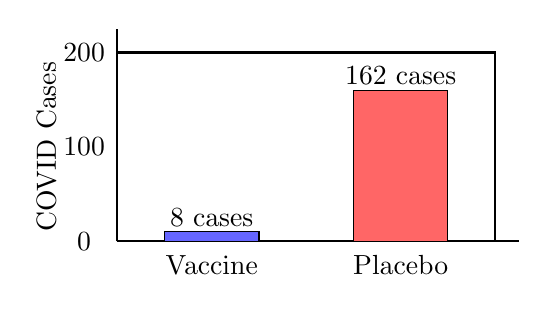
\begin{tikzpicture}[scale=0.6]
			% Bar chart
			\draw[thick] (0,0) -- (8,0) -- (8,4) -- (0,4) -- (0,0);
			\draw[thick] (0,0) -- (0,4.5);
			\draw[thick] (0,0) -- (8.5,0);
			
			% Bars
			\draw[fill=blue!60] (1,0) rectangle (3,0.2);
			\draw[fill=red!60] (5,0) rectangle (7,3.2);
			
			% Labels
			\node at (2, -0.5) {Vaccine};
			\node at (6, -0.5) {Placebo};
			\node at (2, 0.5) {8 cases};
			\node at (6, 3.5) {162 cases};
			
			% Y-axis
			\node at (-0.7, 0) {0};
			\node at (-0.7, 2) {100};
			\node at (-0.7, 4) {200};
			\node[rotate=90] at (-1.5, 2) {COVID Cases};
		\end{tikzpicture}
	\end{frame}
	
	% Slide 26: Ethical Considerations in Human Experiments
	\begin{frame}{Ethical Considerations in Human Experiments}
		\begin{itemize}
			\item \textbf{Ethical constraints} limit what experiments we can perform on humans, even if they would provide clear causal evidence.
			\item We cannot randomly assign people to harmful conditions like smoking, poverty, or dangerous occupations.
			\item All participants must give \textbf{informed consent}, understanding the risks and benefits of participation.
			\item Institutional Review Boards (IRBs) review all human experiments to ensure they meet ethical standards.
		\end{itemize}
		
		\begin{alertblock}{The Ethical Dilemma}
			We might want to know if smoking causes cancer through an RCT, but we cannot ethically randomize people to smoke! This is why we often rely on observational studies for harmful exposures.
		\end{alertblock}
	\end{frame}
	
	% Slide 27: Limitations: When Controlled Experiments Aren't Possible
	\begin{frame}{Limitations: When Controlled Experiments Aren't Possible}
		\begin{itemize}
			\item Some causal questions cannot be answered with RCTs due to practical, ethical, or logical constraints.
			\item \textbf{Practical}: We can't randomly assign countries to different economic systems or planets to different orbits.
			\item \textbf{Ethical}: We can't randomly assign children to different parents or people to natural disasters.
			\item \textbf{Logical}: We can't randomize unchangeable characteristics like biological sex at birth or historical events.
		\end{itemize}
		
		\begin{example}[Questions RCTs Cannot Answer]
			\begin{itemize}
				\item Does democracy cause economic growth?
				\item Do traumatic childhoods cause mental illness?
				\item Did the asteroid impact cause dinosaur extinction?
				\item Does gender affect career advancement?
			\end{itemize}
			For these questions, we need other methods like natural experiments!
		\end{example}
	\end{frame}
	
	% Slide 28: Natural Experiments: When Nature Does the Randomization
	\begin{frame}{Natural Experiments: When Nature Does the Randomization}
		\begin{itemize}
			\item A \textbf{natural experiment} occurs when circumstances naturally create treatment and control groups without researcher intervention.
			\item These "experiments" arise from policy changes, natural disasters, arbitrary boundaries, or other external events.
			\item While not truly random, natural experiments can approximate randomization when assignment is unrelated to outcomes.
			\item Natural experiments help us study causal questions that would be impossible or unethical to test with RCTs.
		\end{itemize}
		
		\begin{block}{Key Advantage}
			Natural experiments allow us to study real-world causation at scales and in contexts where controlled experiments are impossible.
		\end{block}
	\end{frame}
	
	% Slide 29: Example: The Oregon Health Insurance Experiment
	\begin{frame}{Example: The Oregon Health Insurance Experiment}
		\begin{itemize}
			\item In 2008, Oregon used a lottery to allocate limited Medicaid slots among 90,000 low-income adults.
			\item This created a natural experiment: lottery winners (treatment) versus lottery losers (control).
			\item The random lottery approximated the randomization of an RCT without researchers controlling assignment.
			\item Studies found Medicaid coverage increased healthcare use, reduced financial strain, and improved mental health.
		\end{itemize}
		
		\begin{example}[Natural Randomization]
			\begin{tabular}{l|l|l}
				\textbf{Group} & \textbf{Assignment} & \textbf{Outcome Studied} \\
				\hline
				Treatment & Won lottery & Health with Medicaid \\
				Control & Lost lottery & Health without Medicaid \\
				\hline
			\end{tabular}
		\end{example}
	\end{frame}
	
	% Slide 30: Fictional Example: Comparing Gotham and Metropolis Crime Rates
	\begin{frame}{Fictional Example: Comparing Gotham and Metropolis Crime Rates}
		\begin{itemize}
			\item Gotham has Batman while Metropolis has Superman - do different types of heroes cause different crime rates?
			\item This is a natural experiment: cities weren't randomly assigned heroes, but we can still compare outcomes.
			\item \textbf{Challenge}: Cities might differ in other ways (population, economy, corruption) that affect crime.
			\item To make causal claims, we'd need to show the cities were similar before the heroes arrived.
		\end{itemize}
		
		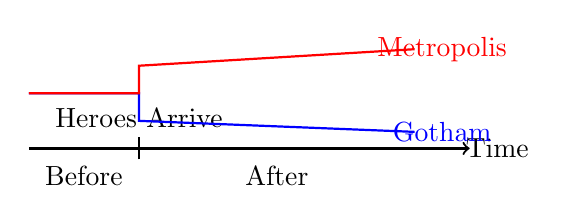
\begin{tikzpicture}[scale=0.7]
			% Timeline
			\draw[thick, ->] (0,0) -- (8,0);
			\node at (8.5, 0) {Time};
			
			% Events
			\draw[thick] (2, -0.2) -- (2, 0.2);
			\node[above] at (2, 0.2) {Heroes Arrive};
			
			% Crime rates
			\draw[thick, blue] (0, 1) -- (2, 1) -- (2, 0.5) -- (7, 0.3);
			\draw[thick, red] (0, 1) -- (2, 1) -- (2, 1.5) -- (7, 1.8);
			
			% Labels
			\node[blue] at (7.5, 0.3) {Gotham};
			\node[red] at (7.5, 1.8) {Metropolis};
			
			% Before/After
			\node at (1, -0.5) {Before};
			\node at (4.5, -0.5) {After};
		\end{tikzpicture}
	\end{frame}
	
	% Slide 31: Real Example: London Cholera Outbreak of 1854
	\begin{frame}{Real Example: London Cholera Outbreak of 1854}
		\begin{itemize}
			\item John Snow used a natural experiment to prove cholera was waterborne, not airborne as believed.
			\item Different London neighborhoods received water from different companies, creating natural treatment groups.
			\item One company's water came from sewage-contaminated Thames; the other's came from cleaner upstream sources.
			\item Deaths clustered in areas served by the contaminated water company, proving water caused cholera transmission.
		\end{itemize}
		
		\begin{alertblock}{Snow's Innovation}
			By mapping deaths and water sources, Snow showed that water supply (not "bad air") caused cholera - revolutionizing public health and establishing epidemiology as a field.
		\end{alertblock}
	\end{frame}
	
	% Slide 32: Strengths and Weaknesses of Natural Experiments
	\begin{frame}{Strengths and Weaknesses of Natural Experiments}
		\begin{itemize}
			\item \textbf{Strengths}: Natural experiments study real-world settings, include entire populations, and examine effects over long time periods.
			\item \textbf{Weaknesses}: Assignment isn't truly random, confounding variables may still exist, and we can't control timing or implementation.
			\item Natural experiments require careful analysis to ensure the "natural" assignment process is truly unrelated to outcomes.
			\item They provide valuable evidence when RCTs are impossible, but generally offer weaker causal evidence than true experiments.
		\end{itemize}
		
		\begin{block}{Comparison with RCTs}
			\begin{tabular}{l|c|c}
				\textbf{Feature} & \textbf{RCT} & \textbf{Natural Experiment} \\
				\hline
				Control & High & Low \\
				External validity & Lower & Higher \\
				Ethical constraints & More & Fewer \\
				Causal certainty & Highest & Moderate \\
			\end{tabular}
		\end{block}
	\end{frame}
	
	% Slide 33: Deductive Reasoning Meets Causal Inference
	\begin{frame}{Deductive Reasoning Meets Causal Inference}
		\begin{itemize}
			\item \textbf{Deductive reasoning} moves from general principles to specific conclusions with logical certainty.
			\item In causal inference, we can deduce: "If A causes B, and B causes C, then A indirectly causes C."
			\item However, most causal claims require empirical evidence, not just logical deduction from premises.
			\item Deduction helps us understand the logical structure of causal chains but can't establish whether causes exist.
		\end{itemize}
		
		\begin{example}[Deductive Causal Chain]
			\begin{enumerate}
				\item Premise 1: Smoking causes lung damage (empirical claim)
				\item Premise 2: Lung damage causes breathing problems (empirical claim)
				\item Conclusion: Therefore, smoking causes breathing problems (deductive inference)
			\end{enumerate}
			The logic is valid, but the premises require empirical support!
		\end{example}
	\end{frame}
	
	% Slide 34: Inductive Reasoning: From Specific Cases to Causal Laws
	\begin{frame}{Inductive Reasoning: From Specific Cases to Causal Laws}
		\begin{itemize}
			\item \textbf{Inductive reasoning} generalizes from specific observations to broader causal principles.
			\item We observe that aspirin relieves headaches in many cases, then inductively infer aspirin causes pain relief generally.
			\item Controlled experiments are essentially systematic inductive reasoning: from sample results to population effects.
			\item The problem of induction applies: we can never be certain our causal laws will hold in all future cases.
		\end{itemize}
		
		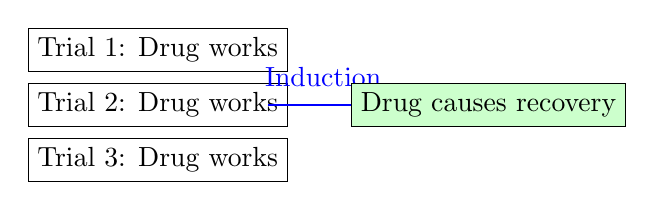
\begin{tikzpicture}[scale=0.7]
			% Specific observations
			\node[draw, rectangle] (obs1) at (0, 0) {Trial 1: Drug works};
			\node[draw, rectangle] (obs2) at (0, -1) {Trial 2: Drug works};
			\node[draw, rectangle] (obs3) at (0, -2) {Trial 3: Drug works};
			
			% Arrow
			\draw[->, thick, blue] (2, -1) -- (4, -1);
			\node[blue] at (3, -0.5) {Induction};
			
			% General law
			\node[draw, rectangle, fill=green!20] (law) at (6, -1) {Drug causes recovery};
		\end{tikzpicture}
	\end{frame}
	
	% Slide 35: Abductive Reasoning: Best Causal Explanations
	\begin{frame}{Abductive Reasoning: Best Causal Explanations}
		\begin{itemize}
			\item \textbf{Abductive reasoning} infers the best causal explanation for observed phenomena.
			\item When we see wet streets, we abductively infer rain as the most likely cause (though sprinklers are possible).
			\item Natural experiments often rely on abduction: we observe patterns and infer the most plausible causal story.
			\item Good abductive causal reasoning considers multiple explanations and chooses the simplest one fitting all evidence.
		\end{itemize}
		
		\begin{alertblock}{Inference to Best Explanation}
			Observation: Students who sit in front get better grades\\
			Possible causes:
			\begin{itemize}
				\item Sitting in front causes better learning (causal)
				\item Motivated students choose front seats (selection)
				\item Teachers favor front-row students (bias)
			\end{itemize}
			Experiments help determine which explanation is best!
		\end{alertblock}
	\end{frame}
	
	% Slide 36: Causal Reasoning: Your New Logical Superpower
	\begin{frame}{Causal Reasoning: Your New Logical Superpower}
		\begin{itemize}
			\item You now have tools to critically evaluate causal claims in science, media, and everyday life.
			\item Remember: correlation isn't causation, confounders lurk everywhere, and good experiments isolate causal effects.
			\item When RCTs aren't possible, natural experiments and careful reasoning can still provide causal insights.
			\item Combine causal thinking with deductive, inductive, and abductive reasoning for comprehensive logical analysis.
		\end{itemize}
		
		\begin{block}{Your Causal Reasoning Toolkit}
			\begin{center}
				$\checkmark$ Identify potential confounders\\
				$\checkmark$ Recognize selection bias\\
				$\checkmark$ Design controlled experiments\\
				$\checkmark$ Spot natural experiments\\
				$\checkmark$ Think counterfactually\\
				$\checkmark$ Integrate with other logical methods
			\end{center}
		\end{block}
	\end{frame}
	
\end{document}